\section{Question about the reference conventions}

\begin{frame}
    \frametitle{LDA+GW theory}
    We always do 
    \begin{equation}
        A_k(\omega) \propto 
        \frac{X}{(\omega - \epsilon_k - \operatorname{Re}\Sigma)^2 + X^2}.
    \end{equation}

    v2 has $X = \operatorname{Im}\Sigma+\eta$, while v1 has just
    $X = \operatorname{Im}\Sigma$. \pause
\begin{enumerate}
    \item To match Loos's result for HF+GW, I need to use v1.
\end{enumerate}

\end{frame}

\begin{frame}
    \frametitle{LDA+GW for 14e/19o}
    \begin{figure}
        \centering
        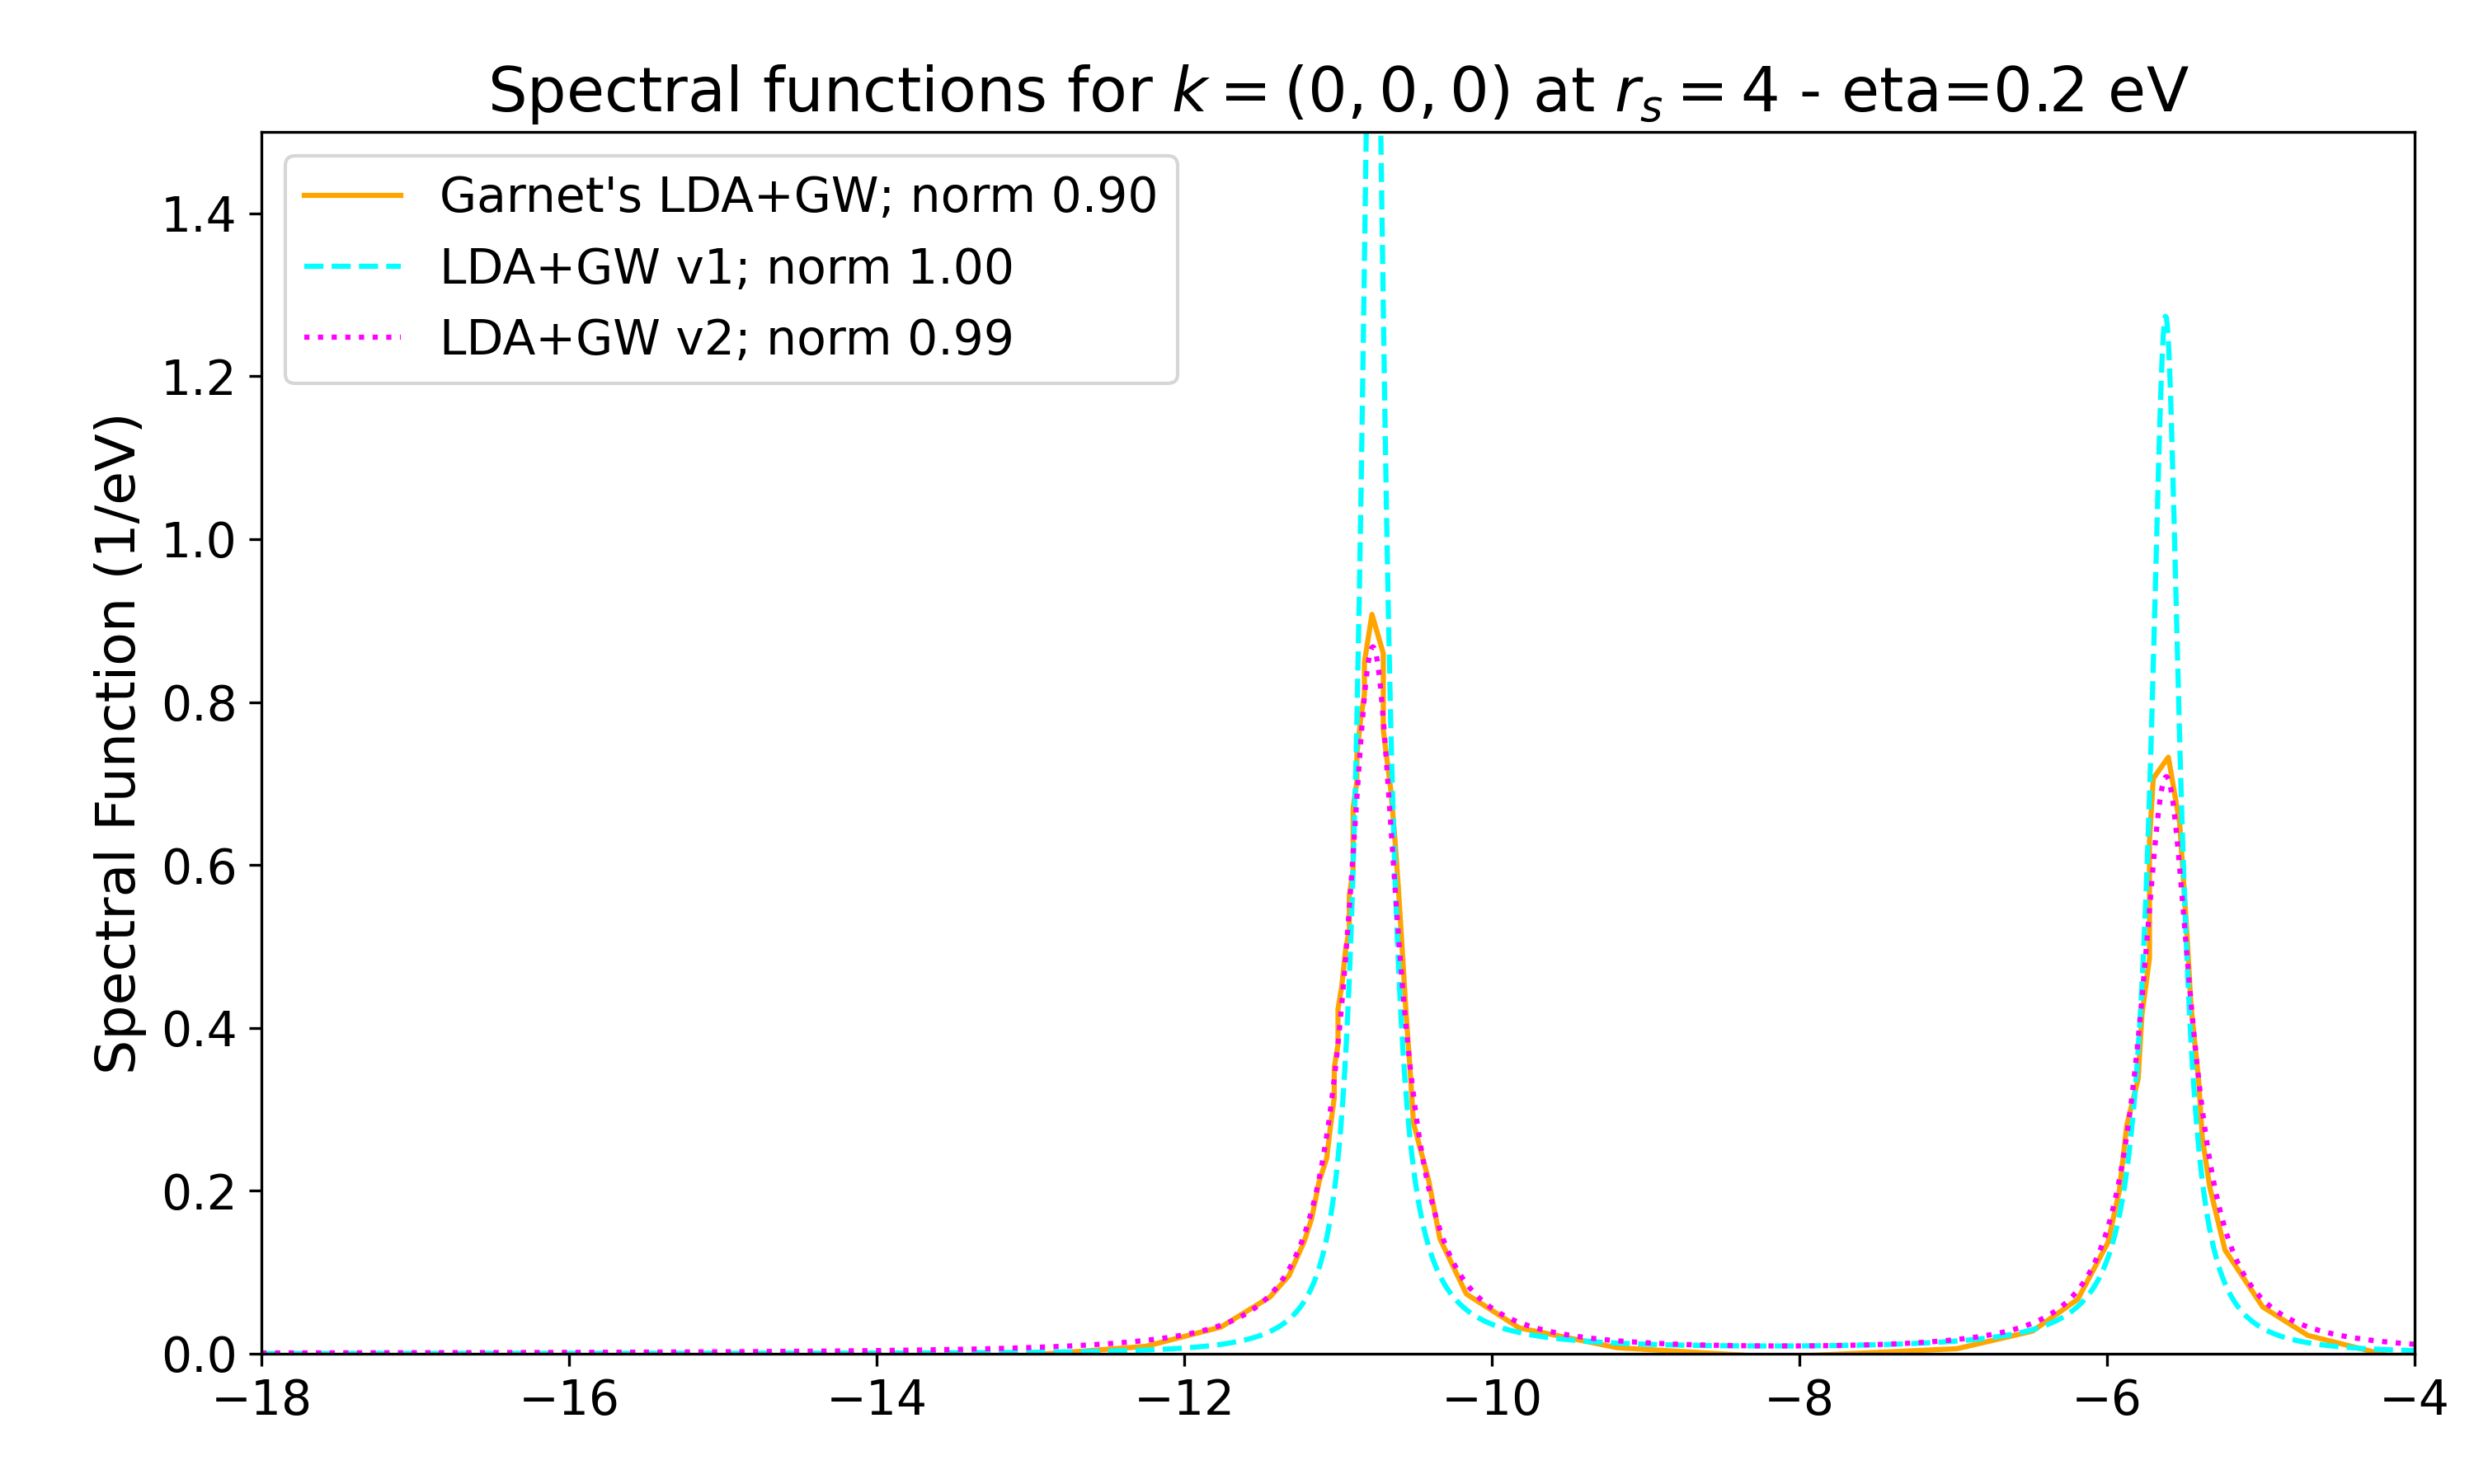
\includegraphics[width=\textwidth]{figs/6-5/gwc_verification.png}
    \end{figure}
\end{frame}

\begin{frame}
    \frametitle{LDA+GW for 114e/485o}
    \begin{figure}
        \centering
        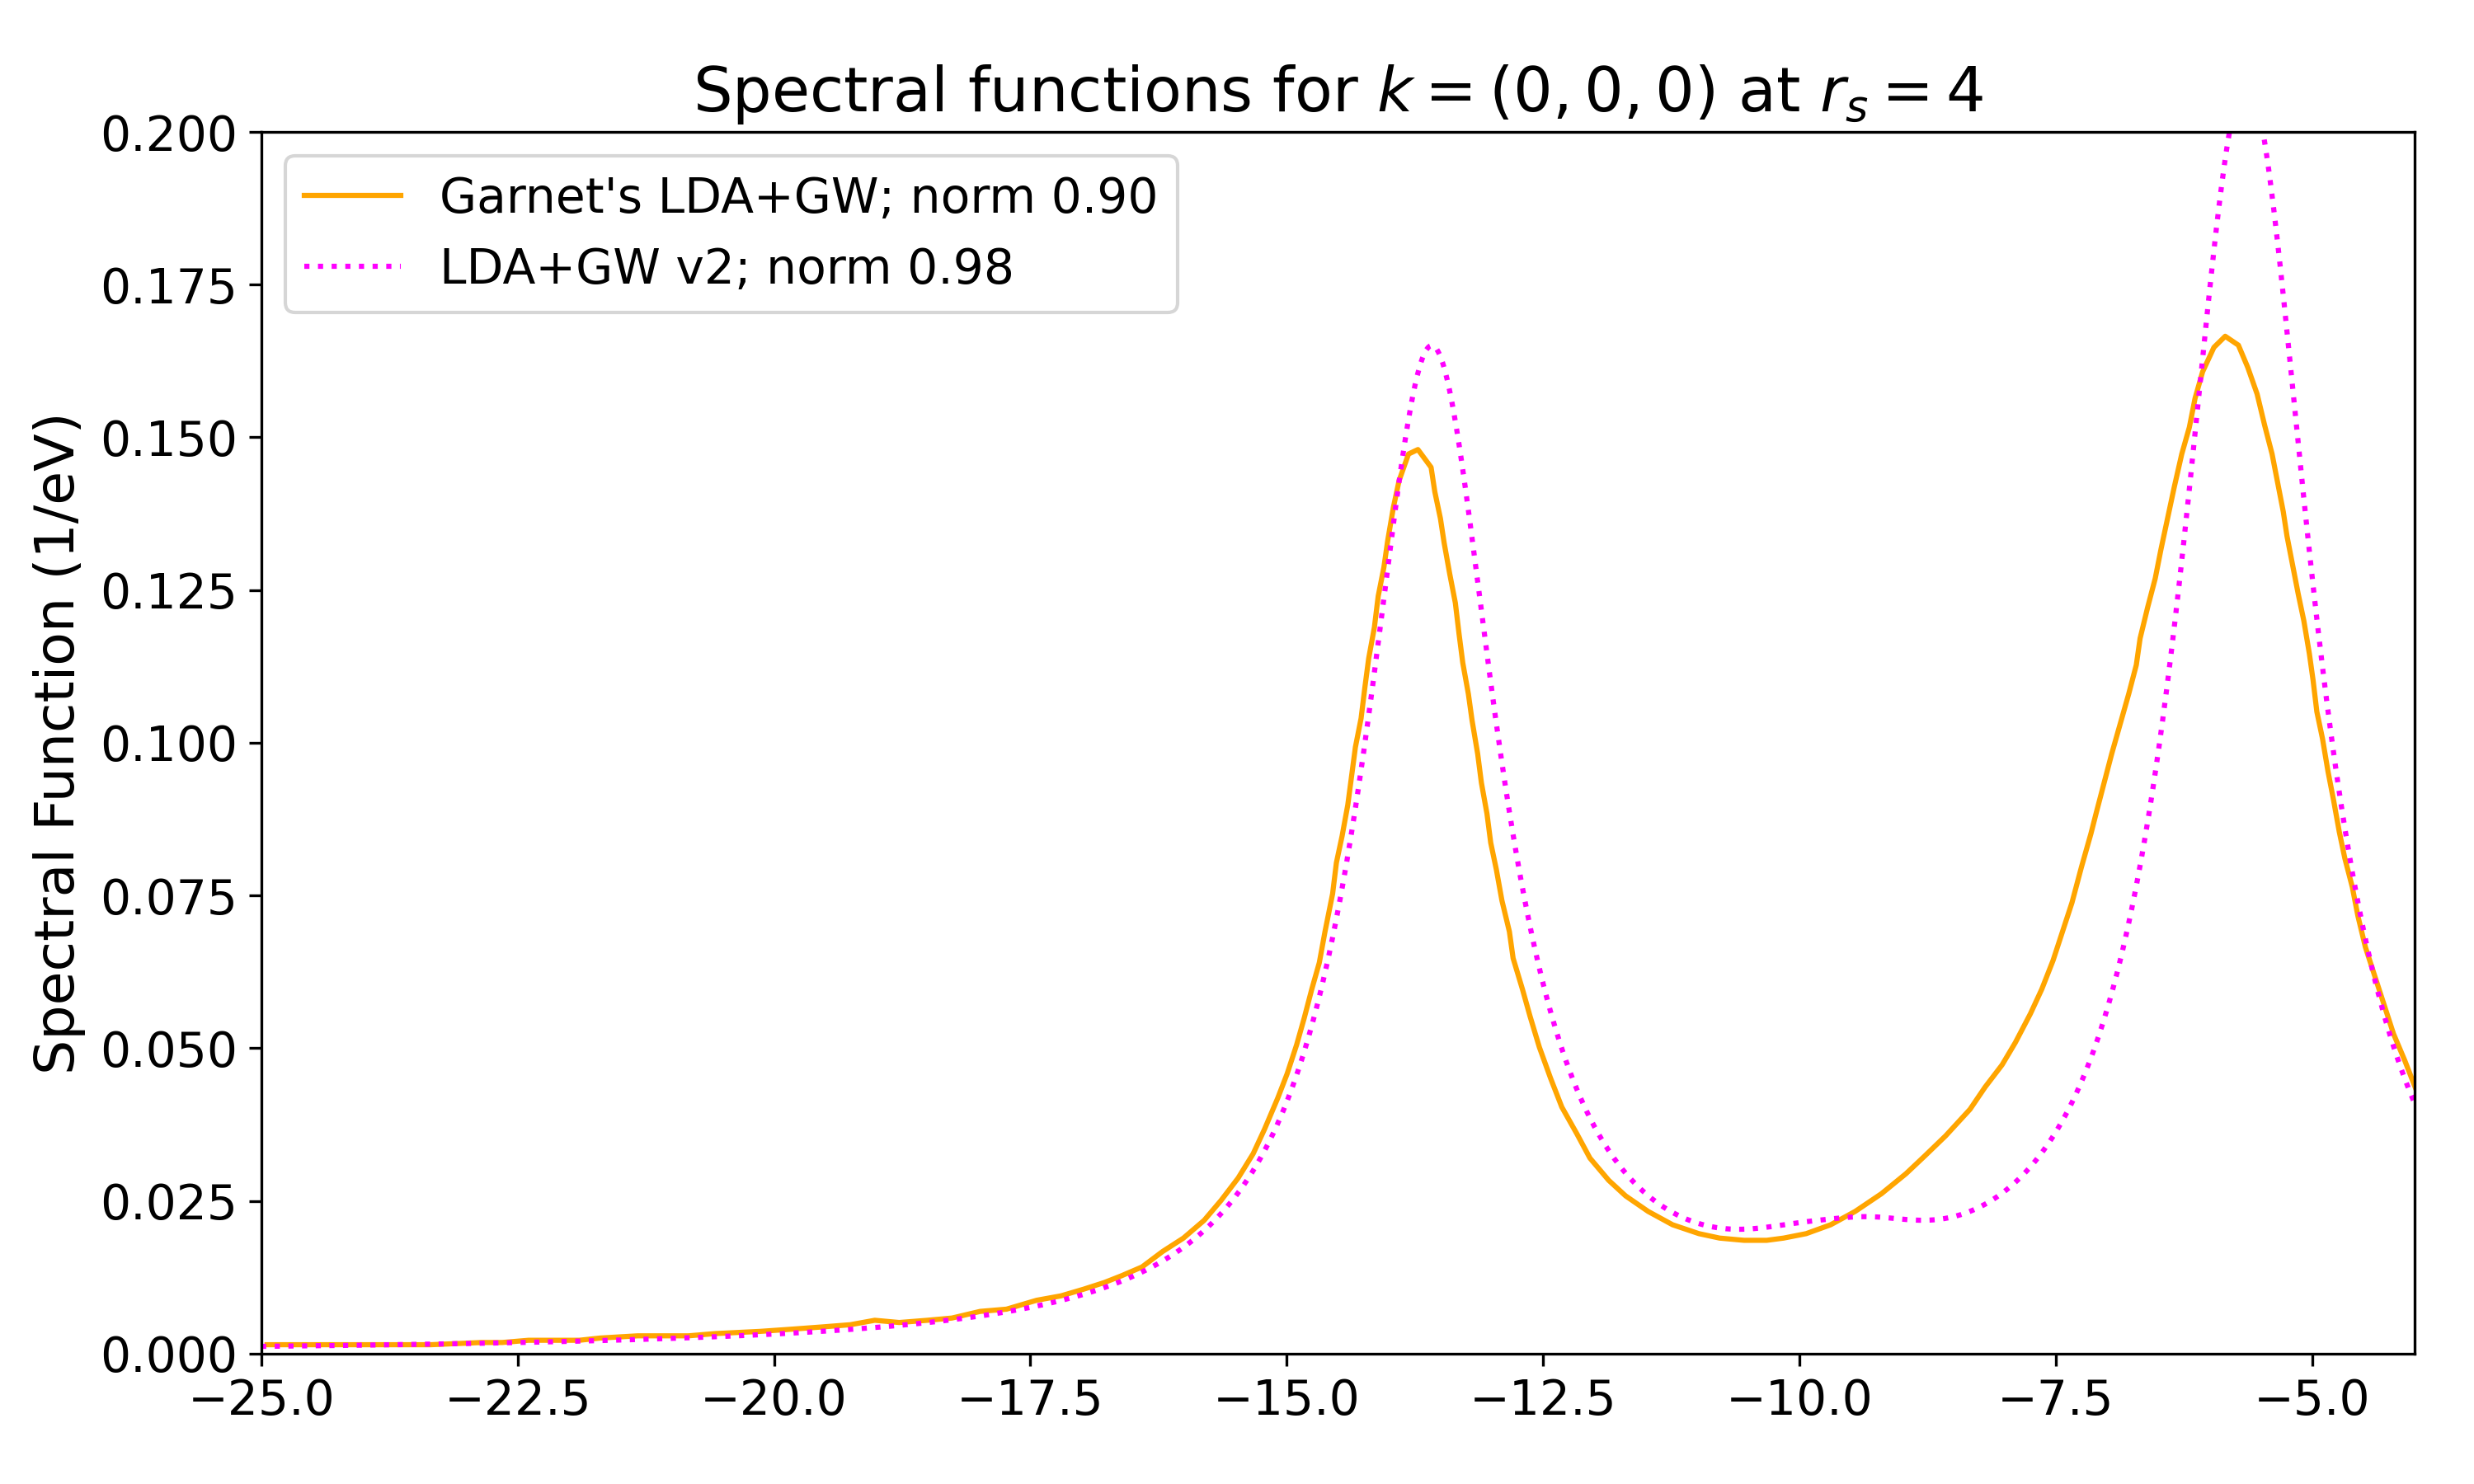
\includegraphics[width=\textwidth]{figs/6-5/gwc_verification_114e.png}
    \end{figure}
\end{frame}

\section{Which single-particle energy to put into the cumulative kernel? }
\begin{frame}
    \frametitle{Theory}
We can do either
\begin{equation}
    C_k^R(t) = i \int \frac{d\omega}{2\pi} e^{-i \omega t} \frac{|\operatorname{Im}\Sigma^R(\omega+\epsilon_k^{QP})|}{(\omega^2)} \left[ e^{-i \omega t} - i \omega t - 1 \right].
\end{equation}
I called this epep@qp \pause
or
\begin{equation}
    C_k^R(t) = i \int \frac{d\omega}{2\pi} e^{-i \omega t} \frac{|\operatorname{Im}\Sigma^R(\omega+\epsilon_k^{MF})|}{(\omega^2)} \left[ e^{-i \omega t} - i \omega t - 1 \right].
\end{equation}
Which I call epep@mf.\pause \\
epe@qp gave the best match with Garnet's 14e/19o
\end{frame}
\begin{frame}
    \frametitle{Results for 114e/485o (GW=G0W0)}
    \begin{figure}
        \centering
        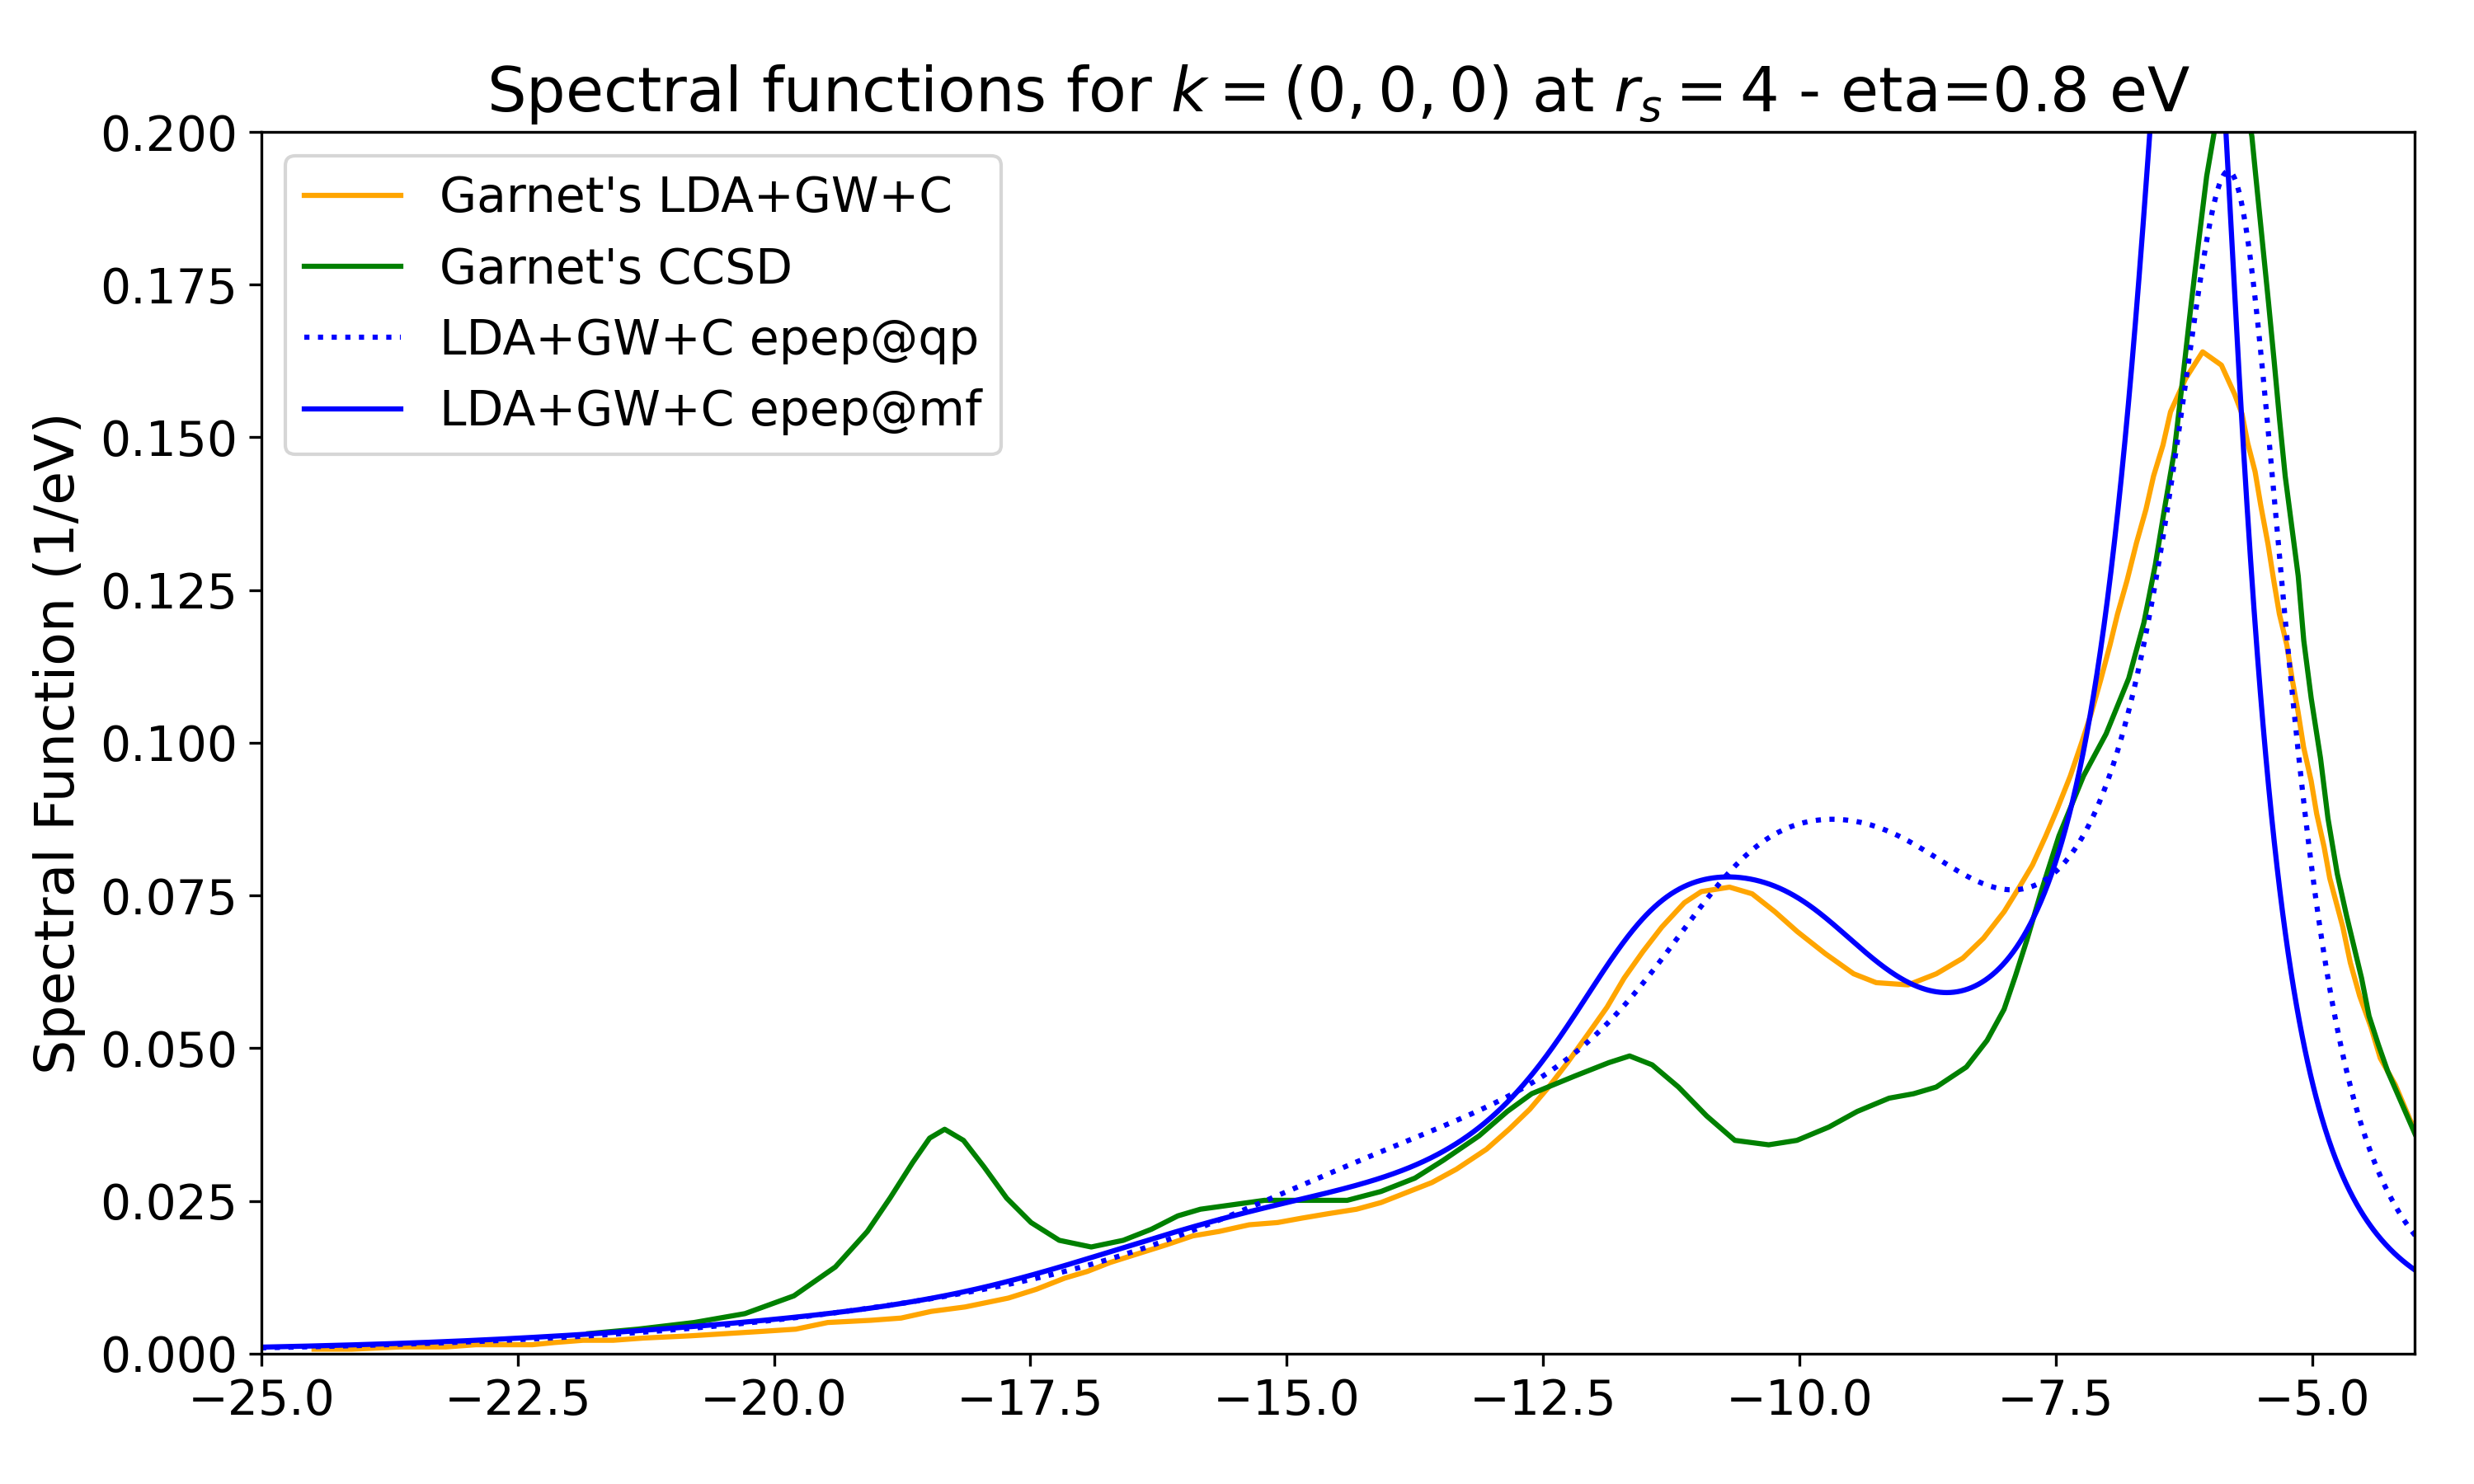
\includegraphics[width=\textwidth]{figs/6-5/epeps.png}
    \end{figure}
\end{frame}
\section{Trying different self-consistent variants }
\begin{frame}
    \frametitle{Theory}
The static part of the cumulant stays the same, but now we have 
\begin{align}
C_k^{R,\text{dyn}}(t)
% i 
% \int \frac{d\omega}{2\pi}
% \frac{e^{-i\omega t}}{(\omega + i\eta)^2}\left[\sum_{i\nu} \frac{\left(M_{ki\nu}^?\right)^2}{\omega +\underbrace{\epsilon_k - \varepsilon_i^? + \Omega_\nu^? + i \eta}_{-\delta_{ki\nu}}} + \sum_{a\nu} \frac{\left(M_{ka\nu}^?\right)^2}{\omega +\underbrace{\epsilon_k - \varepsilon_a^? - \Omega_\nu^? + i \eta}_{-\delta_{ka\nu}}} \right] \\
% % \Delta_k^{\text{static}}t\\
% % &+
% % i 
% % \int \frac{d\omega}{2\pi}
% % \frac{e^{-i\omega t}}{(\omega + i\eta)^2}\left[\sum_{i\nu} \frac{M_{ki\nu}^2}{\omega +\epsilon_k^{\text{LDA}} - \epsilon_i + \Omega_\nu + i \eta} + \sum_{a\nu} \frac{M_{ka\nu}^2}{\omega +\epsilon_k^{\text{LDA}}- \epsilon_a - \Omega_\nu + i \eta} \right] \notag\\
% & =\mathrm{i} \sum_{i v} \left(M_{k i v}^?\right)^2 \int \frac{\mathrm{~d} \omega}{2 \pi} e^{-\mathrm{i} \omega t} \frac{1}{[\omega+\mathrm{i} \eta]^2} \frac{1}{\omega-\delta_{k i v}} +\mathrm{i} \sum_{a v} \left(M_{ka v}^?\right)^2 \int \frac{\mathrm{~d} \omega}{2 \pi} e^{-\mathrm{i} \omega t} \frac{1}{[\omega+\mathrm{i} \eta]^2} \frac{1}{\omega-\delta_{k a v}}
% % & =\mathrm{i} \sum_{i v} M_{k i v}^2 \int \frac{\mathrm{~d} \omega}{2 \pi} e^{-\mathrm{i} \omega t} \frac{1}{[\omega+\mathrm{i} \eta]^2} \frac{1}{\omega-\Delta_{k i v}} +\mathrm{i} \sum_{a v} M_{ka v}^2 \int \frac{\mathrm{~d} \omega}{2 \pi} e^{-\mathrm{i} \omega t} \frac{1}{[\omega+\mathrm{i} \eta]^2} \frac{1}{\omega-\Delta_{k a v}}
% \label{eq:Cpp_1}
% \\
&=
\sum_{i\nu} \zeta_{ki\nu} \left[ e^{-i\delta_{ki\nu} t} - 1 + i\delta_{ki\nu} t \right] + \ldots
\end{align}
where $\zeta_{k i v}=\frac{\left(M_{k i v}^?\right)^2}{\delta_{k i v}^2}$ and $\zeta_{k a v}=\frac{\left(M_{k a v}^?\right)^2}{\delta_{k a v}^2}$ with $\delta_{k i v} = \epsilon_k - \varepsilon_i^? + \Omega_\nu^? + i \eta$ and $\delta_{k a v} = \epsilon_k - \varepsilon_a^? - \Omega_\nu^? + i \eta$ \pause from
\begin{equation}
    \Sigma _k^{c}(\omega)\equiv\sum_{i\nu} \frac{\left(M_{ki\nu}^?\right)^2}{\omega  - \varepsilon_i^{?} + \Omega_\nu^? + i \eta} + \sum_{a\nu} \frac{\left(M_{ka\nu}^?\right)^2}{\omega  - \varepsilon_a^{?} - \Omega_\nu^? + i \eta}
\end{equation}
\end{frame}
\begin{frame}
    \frametitle{Results for epep@qp}
    \begin{figure}
        \centering
        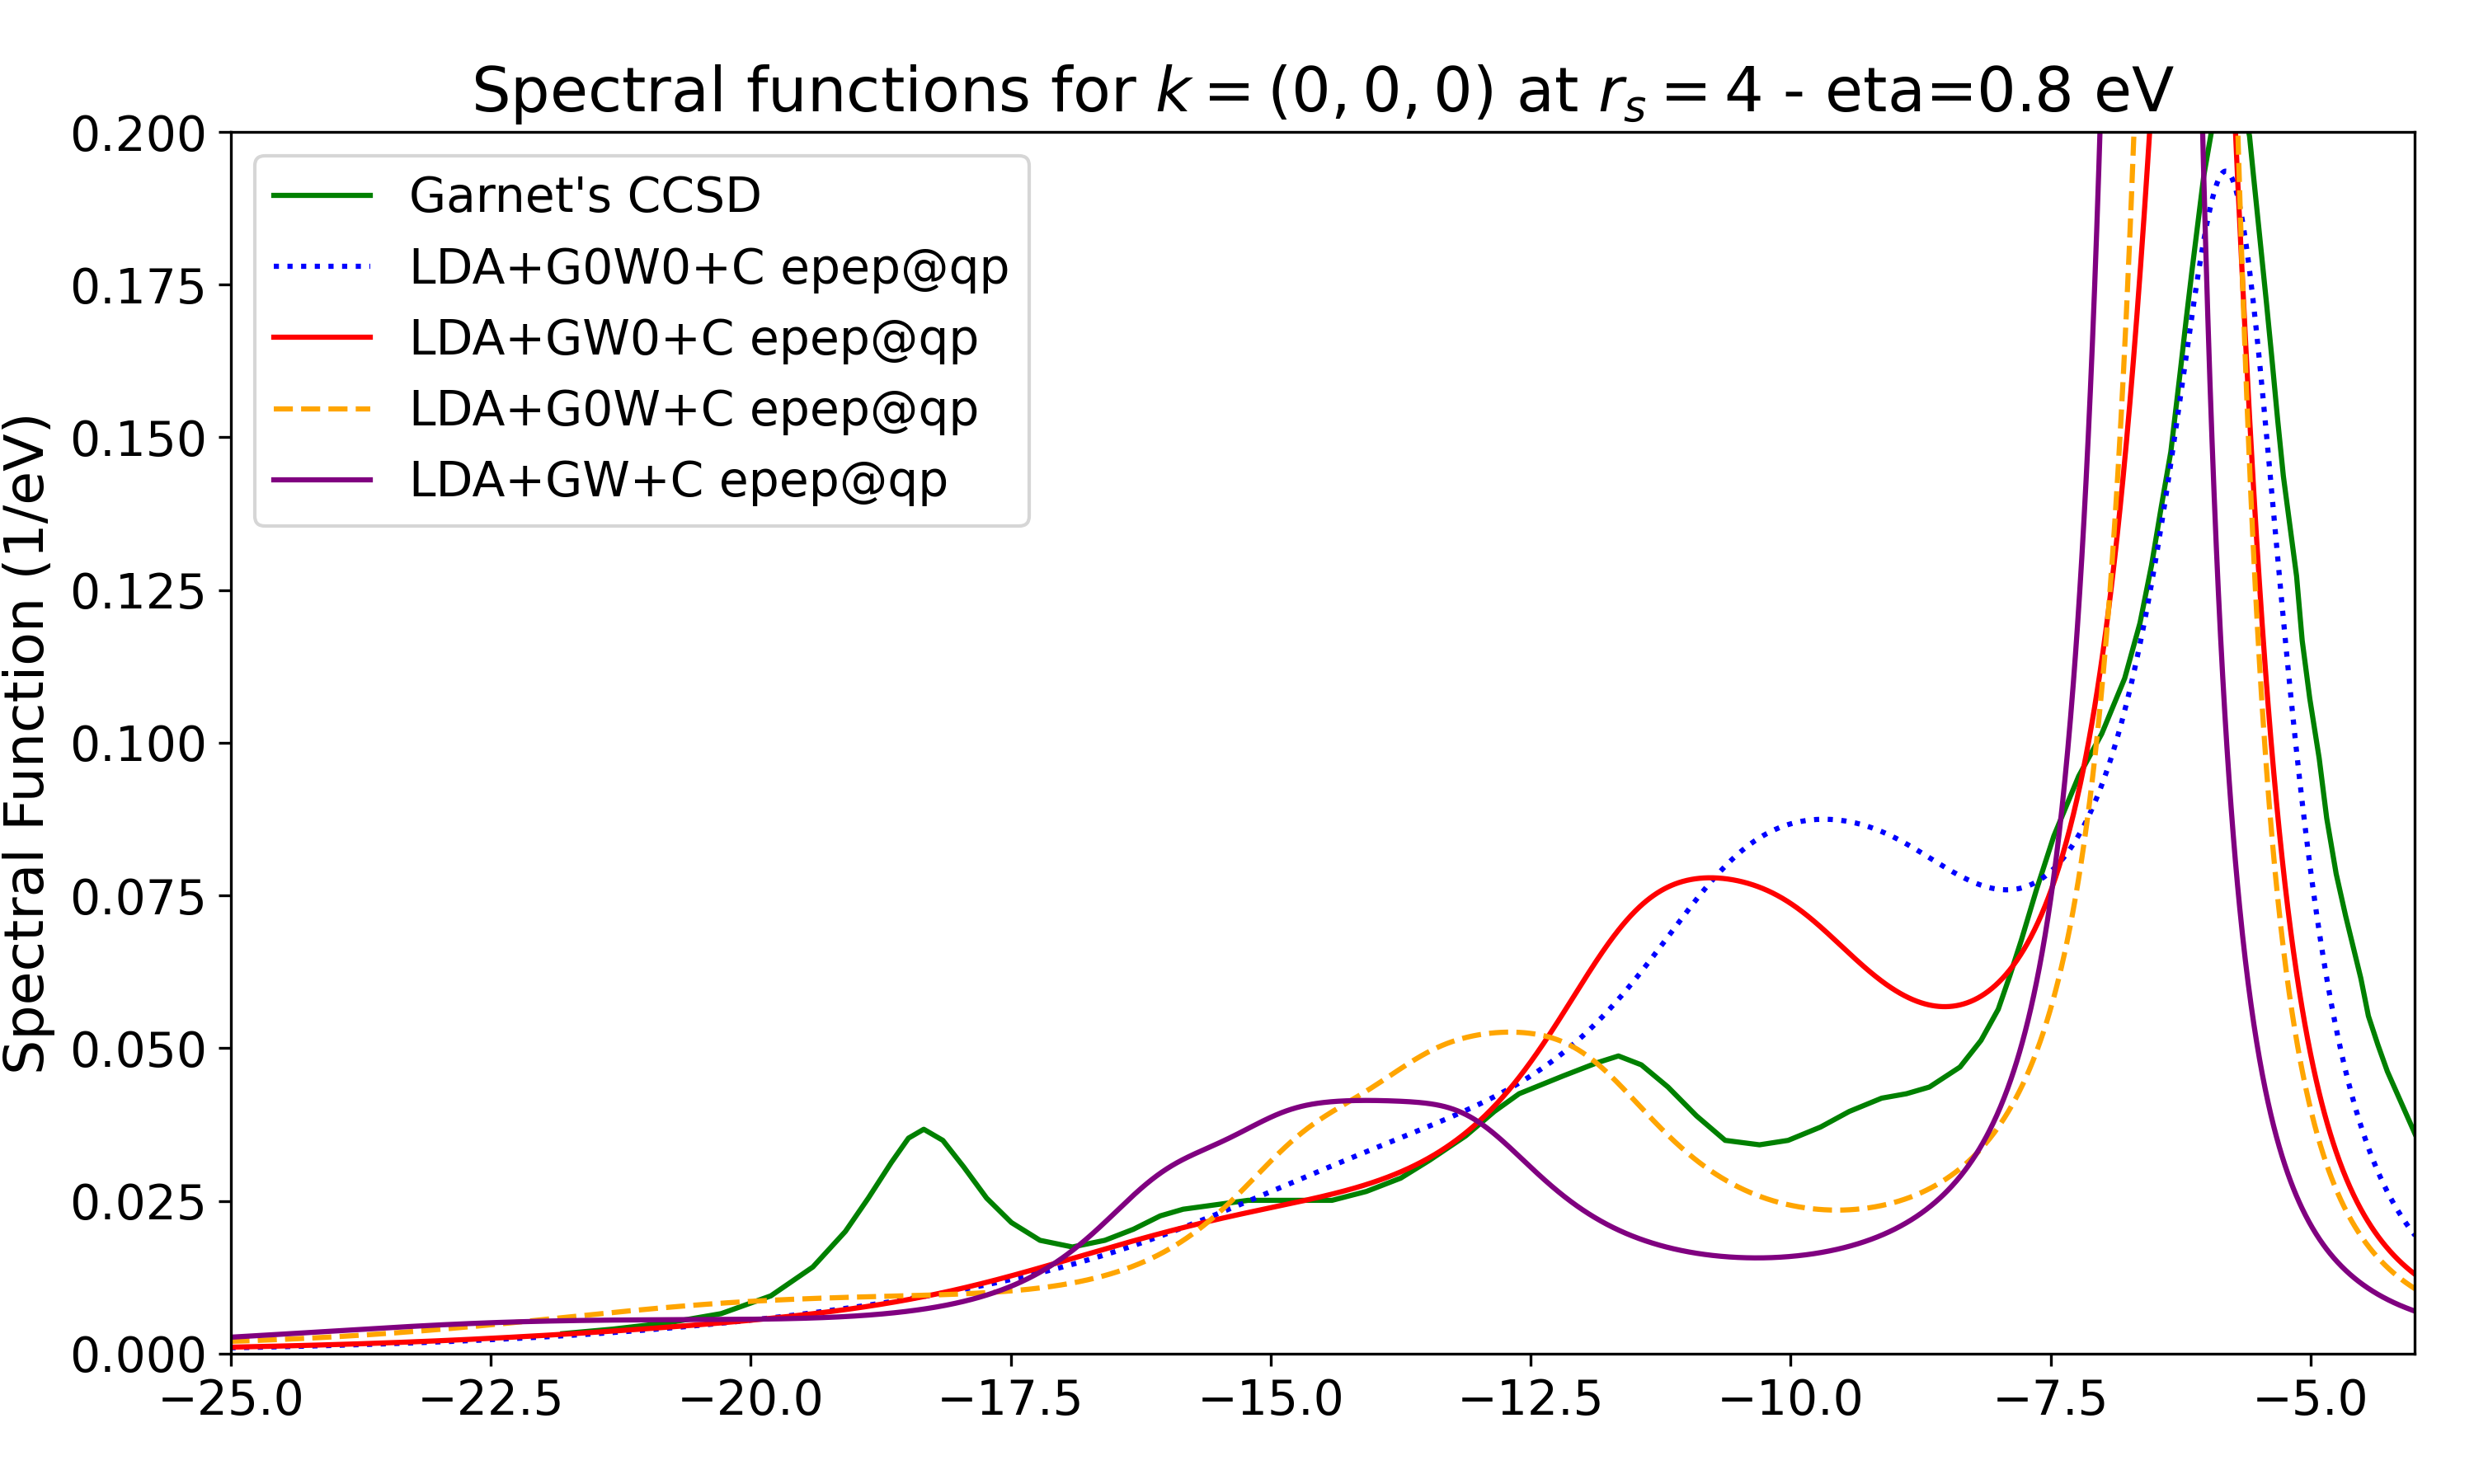
\includegraphics[width=\textwidth]{figs/6-5/scgw_epepqp.png}
    \end{figure}
\end{frame}
\begin{frame}
    \frametitle{Results for epep@mf}
    \begin{figure}
        \centering
        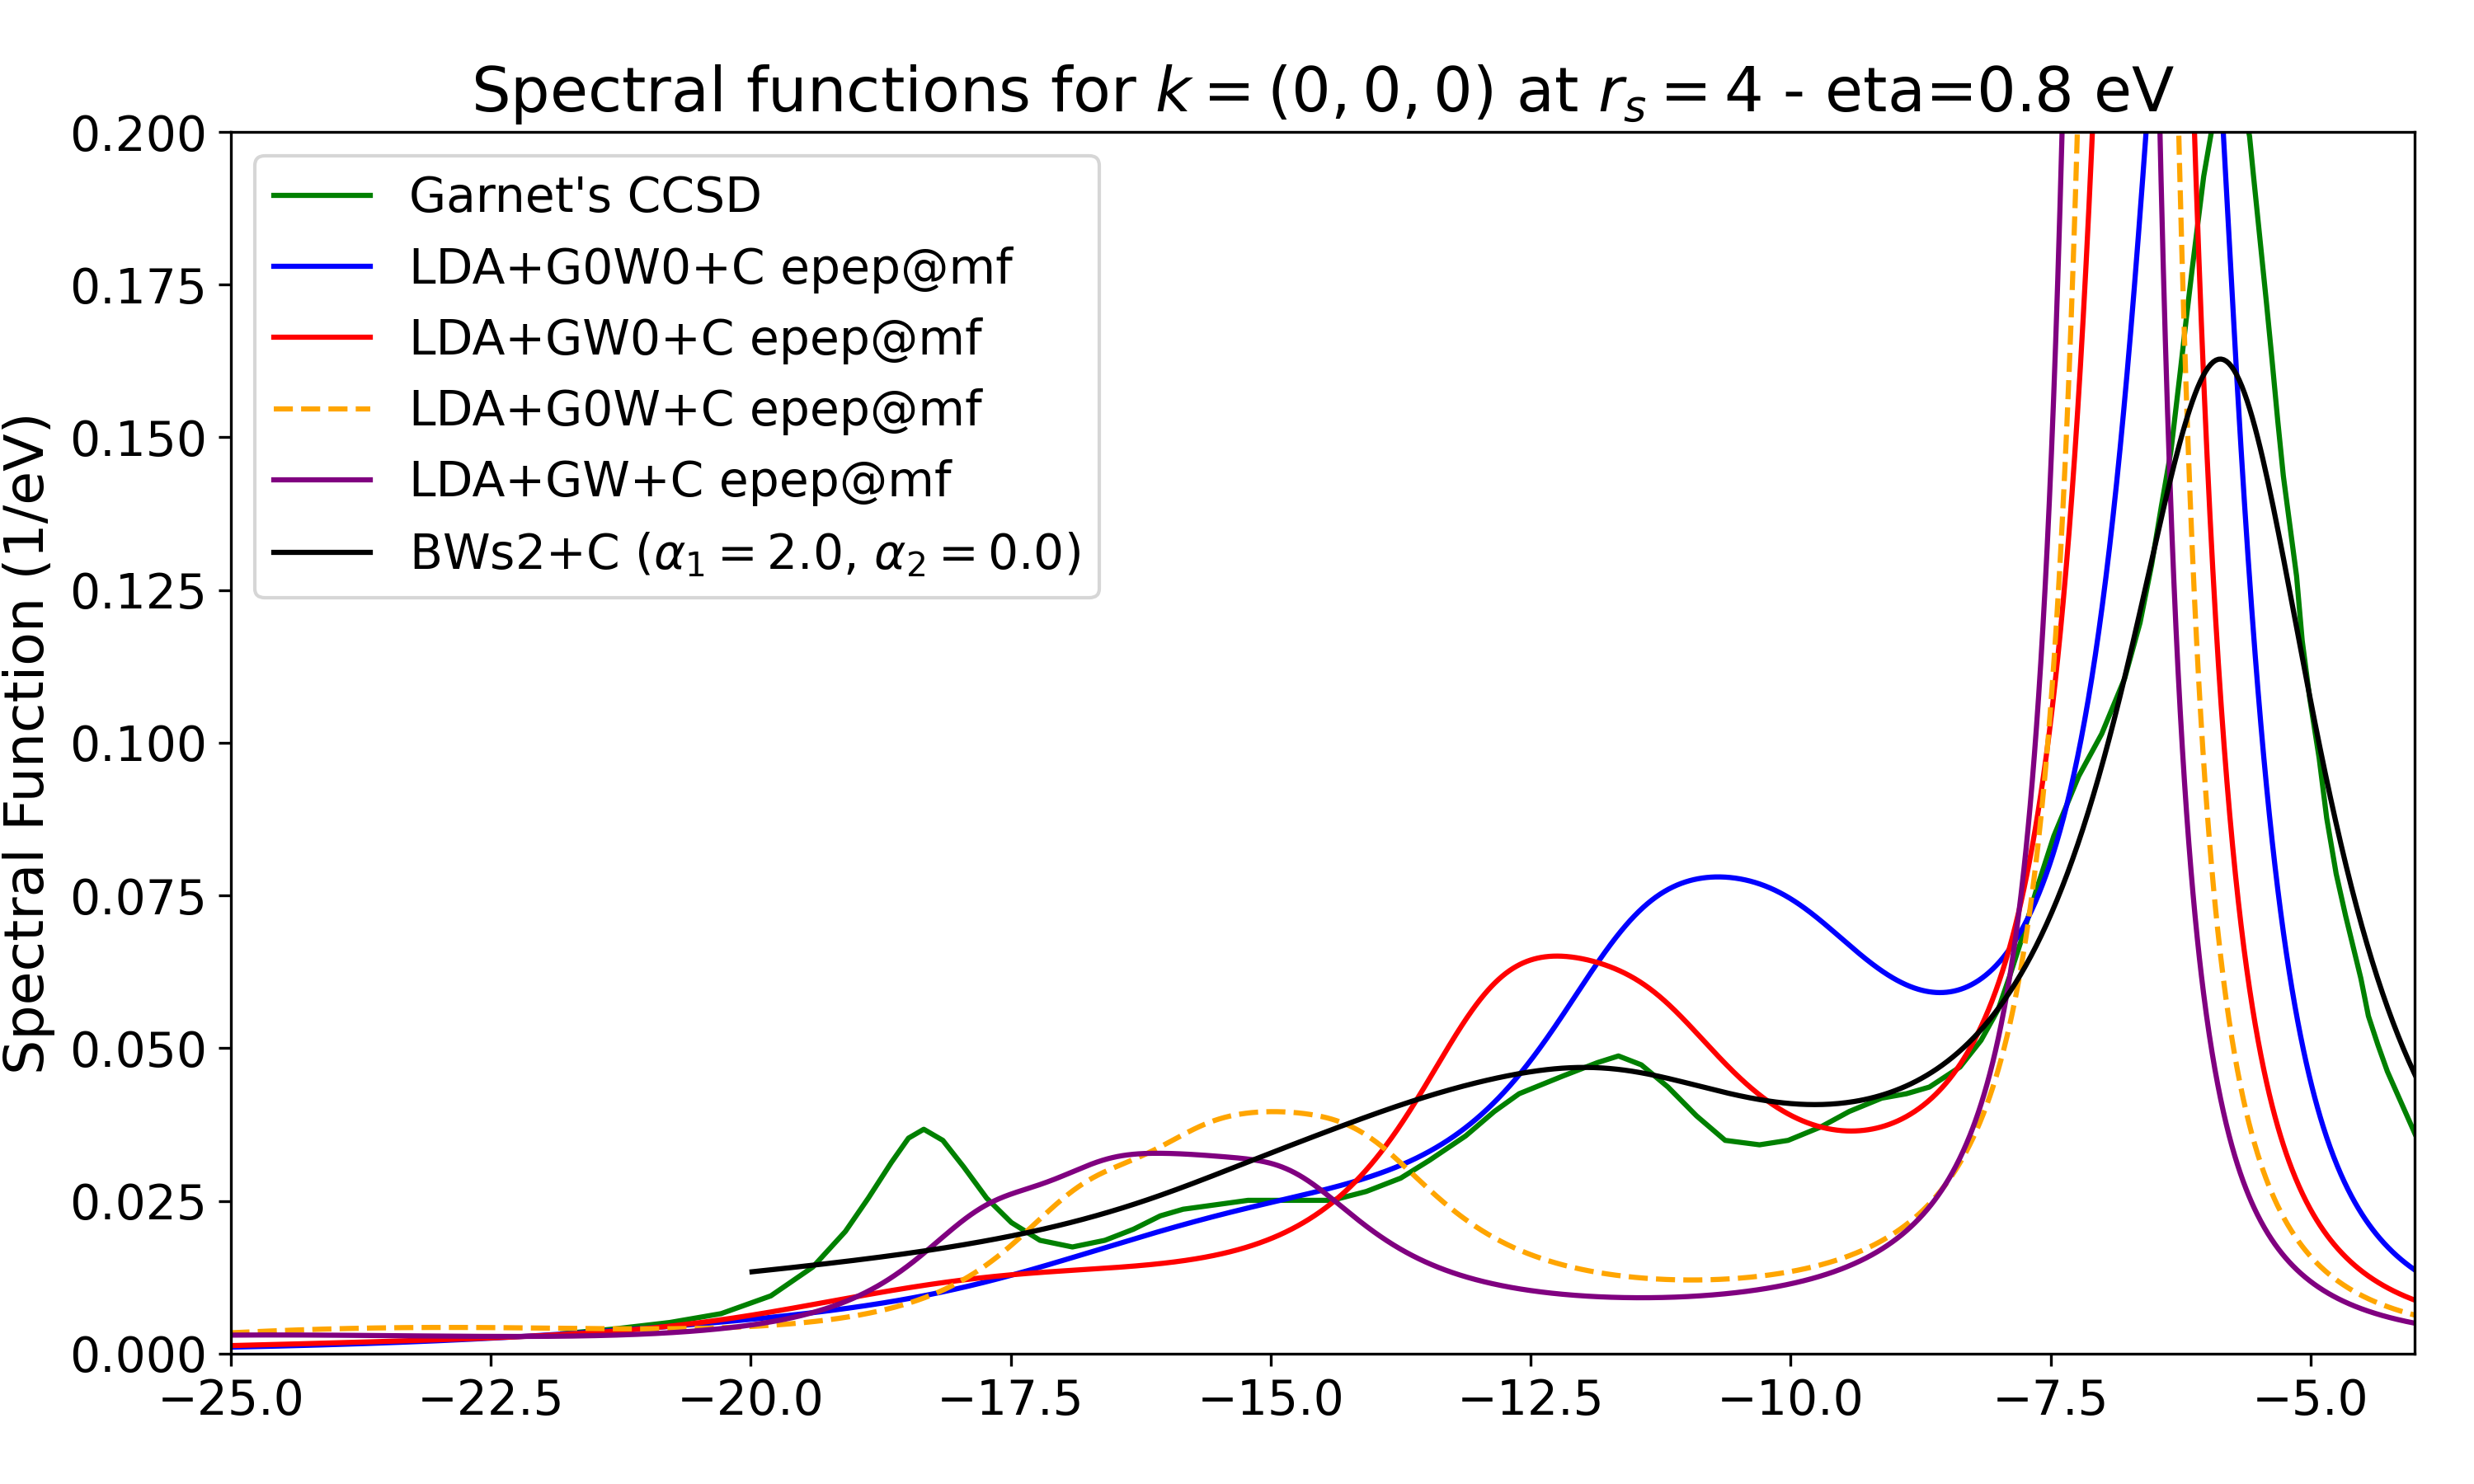
\includegraphics[width=\textwidth]{figs/6-5/scgw_epepmf.png}
    \end{figure}
\end{frame}